\chapter{System Model and Problem Formulation}

\section{Introduction}
This chapter presents the system model and formal problem formulation for temporal-state-aware compact routing in quantum-native entanglement overlay networks. The objective is to extend the existing compact-routing architecture with explicit temporal information associated with each artificial e-link.

The model distinguishes between the physical quantum network and the artificial entanglement overlay. The physical network represents the actual quantum channels, repeaters, memories, and hardware connections. The artificial overlay represents pre-established entangled links between Entanglement Service Providers, which may connect nodes that are not physically adjacent.

The artificial overlay is dynamic because entangled links are generated probabilistically, stored in finite-coherence quantum memories, consumed during entanglement swapping, and regenerated after use or degradation. Therefore, the routing value of an artificial e-link changes over time.

To represent this behavior, each e-link is associated with a temporal state containing its age, initial fidelity, current effective fidelity, coherence time, remaining coherence budget, and regeneration cost. These variables are used to determine whether a structurally valid route is also temporally feasible.

The chapter also defines a time-dependent entangling-cost metric and a temporal entangling-stretch measure. These extensions allow the Partial-Anchor and Full-Anchor compact-routing schemes to be evaluated under heterogeneous age, fidelity, decoherence, and regeneration conditions.

Finally, the routing problem is formulated as the selection of a temporally feasible path that minimizes time-dependent entangling cost while satisfying fidelity, coherence-budget, memory, and compact-routing constraints.
\section{Network Architecture}
The proposed system follows a two-tier quantum-network architecture composed of quantum edge nodes and Entanglement Service Providers. The edge nodes generate application requests, while the Entanglement Service Providers maintain and route shared entanglement across the network core.
\begin{figure}[htbp]
    \centering
    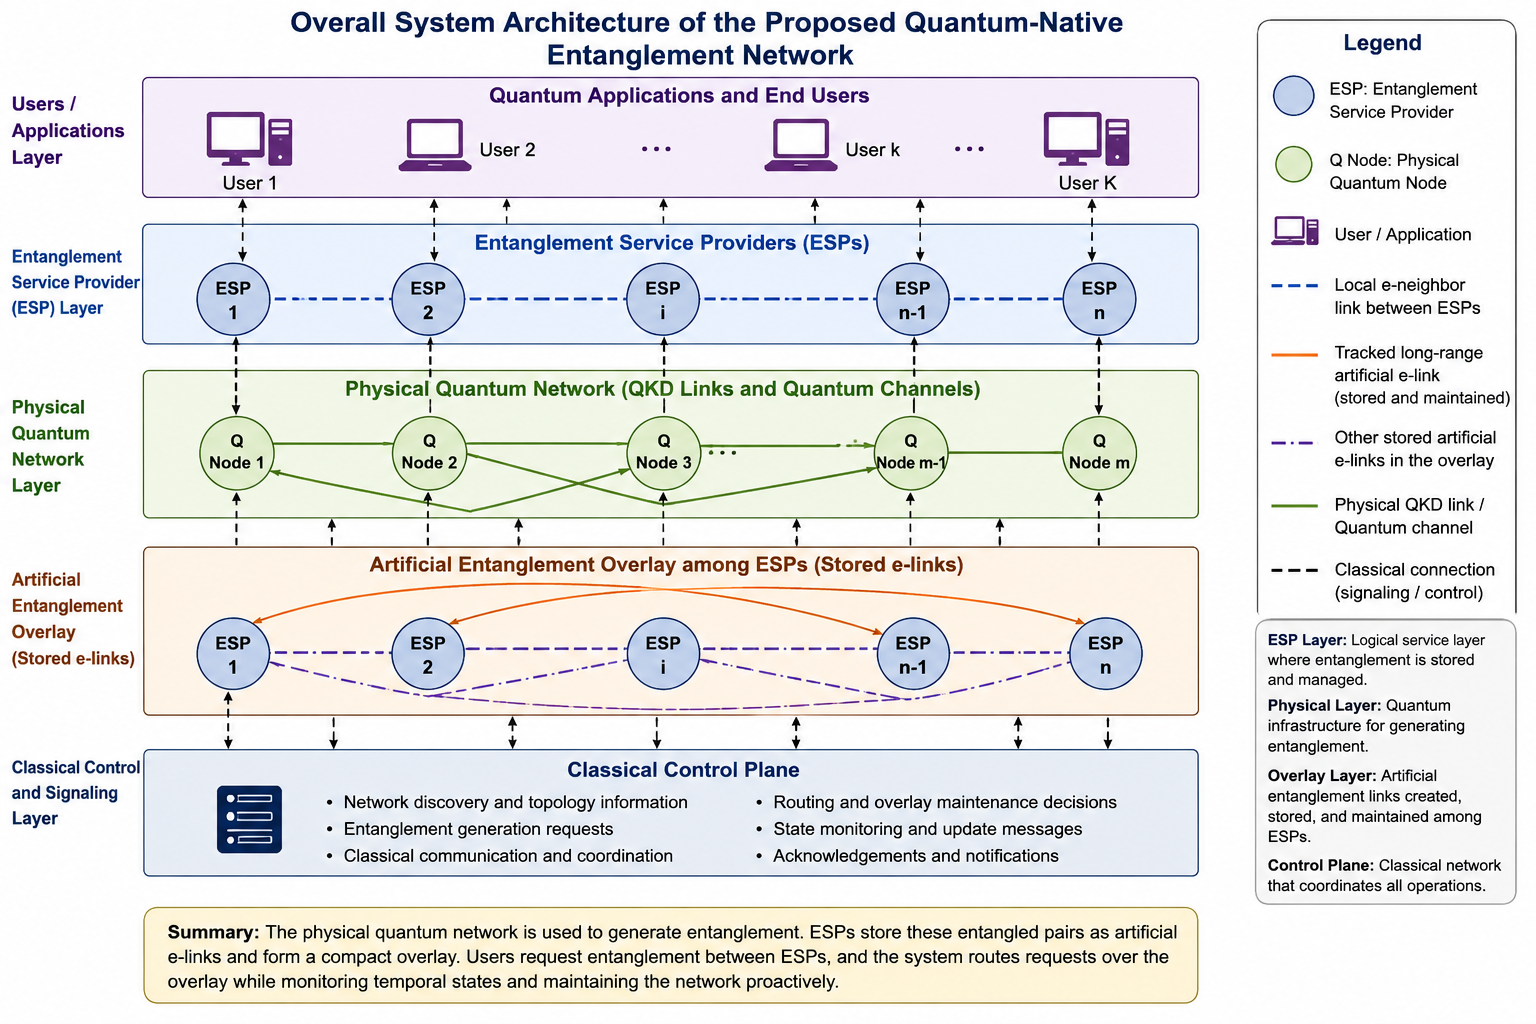
\includegraphics[width=0.95\textwidth]{system_architecture.png}
    \caption{Overall architecture of the quantum-native entanglement network, including the user layer, Entanglement Service Provider layer, physical quantum network, artificial entanglement overlay, and classical control plane.}
    \label{fig:system_architecture}
\end{figure}
Figure~\ref{fig:system_architecture} illustrates the overall layered architecture considered in this thesis.
Let the complete quantum network be represented by

\begin{equation}
    G =
    \left(
    V,E
    \right),
\end{equation}

where $V$ is the set of quantum nodes and $E$ is the set of physical quantum links.

The node set is partitioned into two disjoint subsets:

\begin{equation}
    V
    =
    V_{1}
    \cup
    V_{2},
    \qquad
    V_{1}
    \cap
    V_{2}
    =
    \emptyset,
\end{equation}

where $V_{1}$ contains quantum edge nodes and $V_{2}$ contains Entanglement Service Providers, abbreviated as ESPs.

The number of edge nodes and ESPs is denoted by

\begin{equation}
    |V_{1}| = n_{u},
    \qquad
    |V_{2}| = n_{e},
\end{equation}

such that

\begin{equation}
    |V|
    =
    n
    =
    n_{u}
    +
    n_{e}.
\end{equation}

Each edge node is connected to a serving ESP through a short-range quantum link. The serving ESP receives the end-to-end entanglement request and coordinates the required operations across the tier-2 network.

The ESPs form the quantum-network core. They are equipped with quantum memories, entanglement-generation interfaces, Bell-state measurement modules, and classical communication channels required for heralding and coordination.

An Entanglement-Defined Controller, denoted by $\mathcal{C}_{\mathrm{EDC}}$, manages the control plane. The controller maintains information about artificial e-link availability, routing-table state, link quality, regeneration status, and policy constraints.

The main controller functions are

\begin{itemize}
    \item monitoring artificial e-link availability and temporal state;
    \item constructing and updating e-neighborhoods;
    \item assigning anchor or tracked-link responsibilities;
    \item coordinating route selection;
    \item prioritizing stale-link regeneration;
    \item repairing depleted artificial links; and
    \item enforcing fidelity, memory, and coherence constraints.
\end{itemize}

The architecture separates the physical network from the artificial entanglement overlay. The physical network contains persistent hardware connections, whereas the artificial overlay contains non-persistent entanglement resources established over one or more physical links.

The physical tier-2 network is represented as

\begin{equation}
    G_{\mathrm{P}}
    =
    \left(
    V_{2},
    E_{\mathrm{P}}
    \right),
\end{equation}

where $E_{\mathrm{P}}$ is the set of physical quantum links among ESPs.

The artificial overlay at time $t$ is represented as

\begin{equation}
    G_{\mathrm{A}}(t)
    =
    \left(
    V_{2},
    E_{\mathrm{A}}(t)
    \right),
\end{equation}

where $E_{\mathrm{A}}(t)$ is the set of currently stored artificial e-links.

An artificial e-link

\begin{equation}
    e_{ij}^{\mathrm{A}}(t)
    \in
    E_{\mathrm{A}}(t)
\end{equation}

represents a stored entangled state shared by ESPs $v_i$ and $v_j$. The two ESPs may be physically adjacent or may be connected through a multi-hop entanglement-generation and swapping process.

The artificial overlay is time varying:

\begin{equation}
    E_{\mathrm{A}}(t+1)
    \neq
    E_{\mathrm{A}}(t),
\end{equation}

because artificial e-links may be generated, consumed, discarded, regenerated, or invalidated by decoherence.

The proposed model considers both Partial-Anchor and Full-Anchor compact-routing schemes. In the Partial-Anchor Scheme, every ESP maintains local e-neighbor links, while only selected anchor ESPs maintain long-range artificial links. In the Full-Anchor Scheme, every ESP maintains local e-neighbor links and a selected subset of long-range tracked links.

The architecture assumes that routing decisions are performed using local compact routing-table information, supplemented by temporal-state updates coordinated by the EDC. Persistent complete global knowledge is not required at every ESP.

This architecture provides the structural foundation for defining the physical network model, artificial overlay, temporal e-link state, and coherence-budget-aware routing problem in the following sections.
\section{Physical Quantum Network Model}
The physical quantum network describes the actual hardware-level connectivity among Entanglement Service Providers. It includes optical channels, quantum memories, entanglement sources, Bell-state measurement modules, and classical signaling links required for coordination.

The physical tier-2 network is modeled as an undirected graph

\begin{equation}
    G_{\mathrm{P}}
    =
    \left(
    V_{2},
    E_{\mathrm{P}}
    \right),
\end{equation}

where $V_{2}$ is the set of ESPs and $E_{\mathrm{P}}$ is the set of physical quantum links connecting them.

A physical link between ESPs $v_i$ and $v_j$ is denoted by

\begin{equation}
    e_{ij}^{\mathrm{P}}
    =
    \left(
    v_i,
    v_j
    \right)
    \in
    E_{\mathrm{P}}.
\end{equation}

Each physical link is associated with the parameter set

\begin{equation}
    \Theta_{ij}^{\mathrm{P}}
    =
    \left[
    L_{ij},
    p_{ij}^{\mathrm{gen}},
    F_{ij}^{0},
    T_{2,ij},
    q_{ij},
    M_{ij},
    D_{ij}^{\mathrm{gen}}
    \right],
\end{equation}

where

\begin{itemize}
    \item $L_{ij}$ is the physical distance of the link;
    \item $p_{ij}^{\mathrm{gen}}$ is the elementary-entanglement generation probability;
    \item $F_{ij}^{0}$ is the initial fidelity of a successfully generated pair;
    \item $T_{2,ij}$ is the quantum-memory coherence time;
    \item $q_{ij}$ is the local operational or Bell-state measurement success probability;
    \item $M_{ij}$ is the available quantum-memory capacity; and
    \item $D_{ij}^{\mathrm{gen}}$ is the expected elementary-link generation delay.
\end{itemize}

Time is divided into discrete slots indexed by

\begin{equation}
    t
    \in
    \mathbb{N}.
\end{equation}

For physical link $e_{ij}^{\mathrm{P}}$, the outcome of an elementary-entanglement generation attempt in slot $t$ is represented by

\begin{equation}
    X_{ij}(t)
    \sim
    \mathrm{Bernoulli}
    \left(
    p_{ij}^{\mathrm{gen}}
    \right).
\end{equation}

Therefore,

\begin{equation}
    X_{ij}(t)
    =
    \begin{cases}
        1, & \text{if generation succeeds},\\
        0, & \text{otherwise}.
    \end{cases}
\end{equation}

When $S_{ij}$ parallel modes or generation attempts are available, the probability that at least one pair is generated is

\begin{equation}
    p_{ij}^{\mathrm{link}}
    =
    1
    -
    \left(
    1-p_{ij}^{\mathrm{gen}}
    \right)^{S_{ij}}.
\end{equation}

The elementary-generation probability may depend on the physical distance. A simple loss-based model is

\begin{equation}
    p_{ij}^{\mathrm{gen}}
    =
    \eta_{ij}
    =
    \exp
    \left(
    -\alpha L_{ij}
    \right),
\end{equation}

where $\alpha$ is the channel attenuation coefficient.

Each successful elementary pair occupies one memory unit at both endpoint ESPs. Let

\begin{equation}
    m_i(t)
\end{equation}

denote the number of occupied memory units at ESP $v_i$ in slot $t$. The memory constraint is

\begin{equation}
    m_i(t)
    \leq
    M_i,
    \qquad
    \forall v_i \in V_2.
\end{equation}

A physical route between two ESPs $v_i$ and $v_j$ is represented by

\begin{equation}
    P_{ij}
    =
    \left(
    v_i,
    v_{r_1},
    \ldots,
    v_{r_k},
    v_j
    \right).
\end{equation}

If all elementary links are available and each intermediate Bell-state measurement succeeds independently with probability $q_r$, the approximate end-to-end success probability is

\begin{equation}
    P_{\mathrm{succ}}
    \left(
    P_{ij}
    \right)
    =
    \left(
    \prod_{e_{uv}^{\mathrm{P}} \in P_{ij}}
    p_{uv}^{\mathrm{link}}
    \right)
    \left(
    \prod_{v_r \in P_{ij}\setminus\{v_i,v_j\}}
    q_r
    \right).
\end{equation}

The expected physical-route establishment delay is denoted by

\begin{equation}
    D^{\mathrm{phys}}
    \left(
    P_{ij}
    \right).
\end{equation}

This delay includes elementary-link generation time, classical heralding delay, memory waiting time, purification delay, and swapping delay.

A physical route is considered operationally feasible only if sufficient quantum memories are available and if the expected end-to-end fidelity satisfies

\begin{equation}
    F_{\mathrm{end}}
    \left(
    P_{ij}
    \right)
    \geq
    F_{\min}.
\end{equation}

The physical network provides the substrate for constructing artificial e-links. An artificial e-link between physically non-adjacent ESPs is generated through a feasible physical route and stored at its endpoints.

Therefore, the properties of an artificial e-link depend on the physical route used to create it, including its generation delay, success probability, initial fidelity, memory consumption, and accumulated operational error.
\section{Artificial Entanglement Overlay Model}
The artificial entanglement overlay represents the set of pre-established entangled connections maintained among Entanglement Service Providers. Unlike the physical network, an artificial e-link may connect two ESPs that are not physically adjacent.

At time slot $t$, the artificial overlay is represented by

\begin{equation}
    G_{\mathrm{A}}(t)
    =
    \left(
    V_{2},
    E_{\mathrm{A}}(t)
    \right),
\end{equation}

where $V_{2}$ is the set of ESPs and $E_{\mathrm{A}}(t)$ is the set of artificial e-links available at time $t$.

An artificial e-link between ESPs $v_i$ and $v_j$ is denoted by

\begin{equation}
    e_{ij}^{\mathrm{A}}(t)
    =
    \left(
    v_i,
    v_j
    \right)
    \in
    E_{\mathrm{A}}(t).
\end{equation}

The existence indicator of an artificial e-link is defined as

\begin{equation}
    z_{ij}(t)
    =
    \begin{cases}
        1, & \text{if a usable artificial e-link exists},\\
        0, & \text{otherwise}.
    \end{cases}
\end{equation}

An artificial e-link is considered usable only if it is physically stored, has not been consumed, and satisfies the fidelity requirement

\begin{equation}
    F_{ij}^{\mathrm{eff}}(t)
    \geq
    F_{\min}.
\end{equation}

Artificial e-links are created over physical routes. Let

\begin{equation}
    P_{ij}^{\mathrm{gen}}
\end{equation}

denote the physical path used to establish an artificial e-link between $v_i$ and $v_j$.

The generation success probability of the artificial e-link is

\begin{equation}
    P_{ij}^{\mathrm{A}}
    =
    P_{\mathrm{succ}}
    \left(
    P_{ij}^{\mathrm{gen}}
    \right).
\end{equation}

Its expected generation delay is

\begin{equation}
    D_{ij}^{\mathrm{A}}
    =
    D^{\mathrm{phys}}
    \left(
    P_{ij}^{\mathrm{gen}}
    \right).
\end{equation}

The initial fidelity of the generated artificial e-link is denoted by

\begin{equation}
    F_{ij}^{\mathrm{A},0}.
\end{equation}

This value depends on the fidelities of the elementary pairs, the number of swapping operations, purification operations, and hardware errors encountered during generation.

The artificial overlay changes over time because e-links are generated, stored, consumed, discarded, or regenerated. Its evolution can be expressed as

\begin{equation}
    E_{\mathrm{A}}(t+1)
    =
    \left(
    E_{\mathrm{A}}(t)
    \setminus
    E_{\mathrm{cons}}(t)
    \setminus
    E_{\mathrm{drop}}(t)
    \right)
    \cup
    E_{\mathrm{gen}}(t),
\end{equation}

where

\begin{itemize}
    \item $E_{\mathrm{cons}}(t)$ is the set of e-links consumed during routing or swapping;
    \item $E_{\mathrm{drop}}(t)$ is the set of expired, stale, or unusable e-links; and
    \item $E_{\mathrm{gen}}(t)$ is the set of newly generated or regenerated e-links.
\end{itemize}

Each artificial e-link consumes quantum-memory resources at both endpoint ESPs. Let

\begin{equation}
    n_{ij}^{\mathrm{ebit}}(t)
\end{equation}

denote the number of stored e-bits associated with artificial link $(i,j)$.

The memory constraint at ESP $v_i$ is

\begin{equation}
    \sum_{j:
    e_{ij}^{\mathrm{A}}(t)
    \in
    E_{\mathrm{A}}(t)}
    n_{ij}^{\mathrm{ebit}}(t)
    \leq
    M_i.
\end{equation}

A route over the artificial overlay between source ESP $v_s$ and destination ESP $v_d$ is represented by

\begin{equation}
    R_{s,d}(t)
    =
    \left(
    v_s,
    v_{r_1},
    \ldots,
    v_{r_h},
    v_d
    \right),
\end{equation}

where every consecutive pair must correspond to an available artificial e-link:

\begin{equation}
    e_{uv}^{\mathrm{A}}(t)
    \in
    E_{\mathrm{A}}(t),
    \qquad
    \forall (u,v)
    \in
    R_{s,d}(t).
\end{equation}

The route requires entanglement swapping at each intermediate ESP. Therefore, a route containing $h+1$ artificial links requires $h$ swapping operations.

Assuming independent swapping success probabilities, the route-level success probability is

\begin{equation}
    P_{\mathrm{route}}
    \left(
    R_{s,d}(t)
    \right)
    =
    \left(
    \prod_{(i,j)
    \in
    R_{s,d}(t)}
    z_{ij}(t)
    \right)
    \left(
    \prod_{v_r
    \in
    R_{s,d}(t)\setminus\{v_s,v_d\}}
    q_r
    \right).
\end{equation}

The overlay follows one of two compact-routing structures.

\subsection{Partial-Anchor Overlay}

In the Partial-Anchor Scheme, every ESP maintains artificial e-links with the nodes in its e-neighborhood

\begin{equation}
    \mathcal{N}(v_i).
\end{equation}

A smaller anchor set

\begin{equation}
    \mathcal{T}
    \subseteq
    V_2
\end{equation}

maintains additional long-range artificial links among anchor ESPs.

The artificial-link set can therefore be divided into

\begin{equation}
    E_{\mathrm{A}}^{\mathrm{PA}}(t)
    =
    E_{\mathrm{local}}(t)
    \cup
    E_{\mathrm{anchor}}(t).
\end{equation}

\subsection{Full-Anchor Overlay}

In the Full-Anchor Scheme, every ESP maintains local e-neighbor links and selected long-range tracked links.

The artificial-link set is represented as

\begin{equation}
    E_{\mathrm{A}}^{\mathrm{FA}}(t)
    =
    E_{\mathrm{local}}(t)
    \cup
    E_{\mathrm{tracked}}(t).
\end{equation}

The Full-Anchor Scheme generally provides shorter overlay routes but requires a larger number of ESPs to maintain long-range artificial entanglement.

In both schemes, structural availability alone is insufficient for reliable routing. An artificial e-link may exist in the routing table but may be too old or too close to decoherence to remain usable until route completion.

Therefore, the next section defines an explicit temporal state for every artificial e-link.
\section{Temporal State of Artificial E-Links}
The temporal state of an artificial e-link describes how its routing usefulness changes after generation. Although an e-link may remain stored in quantum memory, its fidelity degrades with time, its expiration risk increases, and its suitability for an end-to-end route may change before it is consumed.

For an artificial e-link shared by ESPs $v_i$ and $v_j$, let

\begin{equation}
    t_{ij}^{\mathrm{gen}}
\end{equation}

denote the time slot in which the link was successfully generated or regenerated.

The age of the e-link at time $t$ is defined as

\begin{equation}
    A_{ij}(t)
    =
    t
    -
    t_{ij}^{\mathrm{gen}}.
\end{equation}

When a new e-link is generated,

\begin{equation}
    A_{ij}(t)
    =
    0.
\end{equation}

If the e-link remains stored and unused, its age evolves as

\begin{equation}
    A_{ij}(t+1)
    =
    A_{ij}(t)
    +
    1.
\end{equation}

If the link is consumed, discarded, or lost, its state is reset to inactive.

Let

\begin{equation}
    x_{ij}(t)
    \in
    \{0,1\}
\end{equation}

denote the activity state of the e-link, where

\begin{equation}
    x_{ij}(t)
    =
    \begin{cases}
        1, & \text{if the e-link is active and stored},\\
        0, & \text{otherwise}.
    \end{cases}
\end{equation}

The complete temporal state of the artificial e-link is defined as

\begin{equation}
    \mathcal{L}_{ij}(t)
    =
    \left[
    x_{ij}(t),
    A_{ij}(t),
    F_{ij}^{\mathrm{A},0},
    F_{ij}^{\mathrm{eff}}(t),
    T_{2,ij},
    B_{ij}(t),
    D_{ij}^{\mathrm{regen}},
    C_{ij}^{\mathrm{regen}}
    \right].
\end{equation}

The components represent

\begin{itemize}
    \item $x_{ij}(t)$: current activity or availability state;
    \item $A_{ij}(t)$: current age of the e-link;
    \item $F_{ij}^{\mathrm{A},0}$: fidelity immediately after generation;
    \item $F_{ij}^{\mathrm{eff}}(t)$: current effective fidelity;
    \item $T_{2,ij}$: coherence time of the stored entanglement;
    \item $B_{ij}(t)$: remaining coherence budget;
    \item $D_{ij}^{\mathrm{regen}}$: expected regeneration delay; and
    \item $C_{ij}^{\mathrm{regen}}$: regeneration resource cost.
\end{itemize}

The temporal state is updated at the beginning of every time slot. If no generation, consumption, or discard action occurs, the link ages and its effective fidelity is recomputed.

A generic state-update rule is

\begin{equation}
    \mathcal{L}_{ij}(t+1)
    =
    \begin{cases}
        \mathcal{L}_{ij}^{\mathrm{new}},
        & \text{if generation succeeds},\\
        \mathcal{L}_{ij}^{\mathrm{age}},
        & \text{if the link remains stored},\\
        \mathcal{L}_{ij}^{\mathrm{inactive}},
        & \text{if consumed, discarded, or expired}.
    \end{cases}
\end{equation}

For a newly generated link,

\begin{equation}
    \mathcal{L}_{ij}^{\mathrm{new}}
    =
    \left[
    1,
    0,
    F_{ij}^{\mathrm{A},0},
    F_{ij}^{\mathrm{A},0},
    T_{2,ij},
    B_{ij}^{0},
    D_{ij}^{\mathrm{regen}},
    C_{ij}^{\mathrm{regen}}
    \right].
\end{equation}

For an aged but still active link,

\begin{equation}
    \mathcal{L}_{ij}^{\mathrm{age}}
    =
    \left[
    1,
    A_{ij}(t)+1,
    F_{ij}^{\mathrm{A},0},
    F_{ij}^{\mathrm{eff}}(t+1),
    T_{2,ij},
    B_{ij}(t+1),
    D_{ij}^{\mathrm{regen}},
    C_{ij}^{\mathrm{regen}}
    \right].
\end{equation}

An artificial e-link is declared stale when at least one of the following conditions holds:

\begin{equation}
    F_{ij}^{\mathrm{eff}}(t)
    <
    F_{\min},
\end{equation}

\begin{equation}
    B_{ij}(t)
    \leq
    0,
\end{equation}

or

\begin{equation}
    A_{ij}(t)
    \geq
    A_{ij}^{\max},
\end{equation}

where $A_{ij}^{\max}$ is a maximum allowed storage age.

The stale-link indicator is defined as

\begin{equation}
    s_{ij}(t)
    =
    \begin{cases}
        1, & \text{if the e-link is stale},\\
        0, & \text{otherwise}.
    \end{cases}
\end{equation}

A stale link may still physically exist in memory, but it is excluded from temporally feasible routes.

The usable-link indicator is therefore

\begin{equation}
    u_{ij}(t)
    =
    x_{ij}(t)
    \left(
    1-s_{ij}(t)
    \right).
\end{equation}

The temporally usable artificial overlay is then

\begin{equation}
    G_{\mathrm{U}}(t)
    =
    \left(
    V_2,
    E_{\mathrm{U}}(t)
    \right),
\end{equation}

where

\begin{equation}
    E_{\mathrm{U}}(t)
    =
    \left\{
    e_{ij}^{\mathrm{A}}(t)
    \in
    E_{\mathrm{A}}(t)
    :
    u_{ij}(t)=1
    \right\}.
\end{equation}

This distinction between stored and temporally usable links is essential. A compact routing table may contain an entry for an e-link that is no longer safe for end-to-end routing.

The proposed routing framework therefore performs path selection over $G_{\mathrm{U}}(t)$ rather than over the complete stored overlay $G_{\mathrm{A}}(t)$.
\section{Fidelity and Decoherence Model}
The fidelity and decoherence model describes how the quality of an artificial e-link changes during generation, storage, purification, and swapping. Since the proposed routing framework relies on stored entanglement, temporal fidelity degradation must be represented explicitly.

For an artificial e-link shared between ESPs $v_i$ and $v_j$, let

\begin{equation}
    F_{ij}^{\mathrm{A},0}
\end{equation}

denote the fidelity immediately after the e-link is generated.

The initial fidelity depends on the physical route used for generation, the quality of the elementary entangled pairs, swapping operations, purification operations, and hardware errors.

The effective fidelity of the stored e-link at time $t$ is denoted by

\begin{equation}
    F_{ij}^{\mathrm{eff}}(t).
\end{equation}

A general temporal-fidelity model can be expressed as

\begin{equation}
    F_{ij}^{\mathrm{eff}}(t)
    =
    f_{\mathrm{dec}}
    \left(
    F_{ij}^{\mathrm{A},0},
    A_{ij}(t),
    T_{2,ij},
    \epsilon_{ij}^{\mathrm{op}}
    \right),
\end{equation}

where $\epsilon_{ij}^{\mathrm{op}}$ represents accumulated operational error.

For simulation, a simplified exponential model may be used:

\begin{equation}
    F_{ij}^{\mathrm{eff}}(t)
    =
    F_{\infty}
    +
    \left(
    F_{ij}^{\mathrm{A},0}
    -
    F_{\infty}
    \right)
    \exp
    \left(
    -\frac{A_{ij}(t)\Delta}{T_{2,ij}}
    \right),
\end{equation}

where

\begin{itemize}
    \item $\Delta$ is the duration of one time slot;
    \item $T_{2,ij}$ is the coherence time; and
    \item $F_{\infty}$ is the asymptotic fidelity under the selected noise model.
\end{itemize}

For a two-qubit Werner-state approximation, the asymptotic fidelity is commonly taken as

\begin{equation}
    F_{\infty}
    =
    \frac{1}{4}.
\end{equation}

Therefore, the storage-decay model becomes

\begin{equation}
    F_{ij}^{\mathrm{eff}}(t)
    =
    \frac{1}{4}
    +
    \left(
    F_{ij}^{\mathrm{A},0}
    -
    \frac{1}{4}
    \right)
    \exp
    \left(
    -\frac{A_{ij}(t)\Delta}{T_{2,ij}}
    \right).
\end{equation}

This formulation ensures that fidelity gradually approaches the fully mixed two-qubit-state fidelity rather than incorrectly approaching zero.

An equivalent formulation can be written using the Werner parameter

\begin{equation}
    p_{ij}^{W}(t)
    =
    \frac{
    4F_{ij}^{\mathrm{eff}}(t)-1
    }{3}.
\end{equation}

The initial Werner parameter is

\begin{equation}
    p_{ij}^{W,0}
    =
    \frac{
    4F_{ij}^{\mathrm{A},0}-1
    }{3}.
\end{equation}

Under exponential storage decay,

\begin{equation}
    p_{ij}^{W}(t)
    =
    p_{ij}^{W,0}
    \exp
    \left(
    -\frac{A_{ij}(t)\Delta}{T_{2,ij}}
    \right).
\end{equation}

The corresponding effective fidelity is recovered as

\begin{equation}
    F_{ij}^{\mathrm{eff}}(t)
    =
    \frac{
    1+3p_{ij}^{W}(t)
    }{4}.
\end{equation}

Consider an artificial-overlay route

\begin{equation}
    R_{s,d}(t)
    =
    \left(
    v_s,
    v_{r_1},
    \ldots,
    v_{r_h},
    v_d
    \right).
\end{equation}

Let the route contain the artificial e-link set

\begin{equation}
    E
    \left(
    R_{s,d}(t)
    \right).
\end{equation}

Under the Werner approximation, the route-level parameter before accounting for swapping errors is

\begin{equation}
    p_{\mathrm{route}}^{W}(t)
    =
    \prod_{
    (i,j)
    \in
    E(R_{s,d}(t))
    }
    p_{ij}^{W}(t).
\end{equation}

To account for imperfect swapping operations, let

\begin{equation}
    \lambda_r
    \in
    [0,1]
\end{equation}

denote the fidelity-retention factor of the Bell-state measurement at intermediate ESP $v_r$.

The end-to-end Werner parameter is then approximated by

\begin{equation}
    p_{s,d}^{W,\mathrm{end}}(t)
    =
    \left(
    \prod_{
    (i,j)
    \in
    E(R_{s,d}(t))
    }
    p_{ij}^{W}(t)
    \right)
    \left(
    \prod_{
    v_r
    \in
    R_{s,d}(t)\setminus\{v_s,v_d\}
    }
    \lambda_r
    \right).
\end{equation}

The resulting end-to-end fidelity is

\begin{equation}
    F_{s,d}^{\mathrm{end}}(t)
    =
    \frac{
    1
    +
    3p_{s,d}^{W,\mathrm{end}}(t)
    }{4}.
\end{equation}

A route satisfies the fidelity requirement only if

\begin{equation}
    F_{s,d}^{\mathrm{end}}(t)
    \geq
    F_{\min}.
\end{equation}

However, evaluating fidelity only at the route-selection time is insufficient. Additional delay may occur before all swapping operations are completed.

Let

\begin{equation}
    \widehat{D}_{s,d}^{\mathrm{route}}(t)
\end{equation}

denote the predicted route-completion delay.

The predicted fidelity of e-link $(i,j)$ at consumption time is

\begin{equation}
    \widehat{F}_{ij}^{\mathrm{cons}}(t)
    =
    \frac{1}{4}
    +
    \left(
    F_{ij}^{\mathrm{eff}}(t)
    -
    \frac{1}{4}
    \right)
    \exp
    \left(
    -\frac{
    \widehat{D}_{ij}^{\mathrm{use}}(t)
    }{
    T_{2,ij}
    }
    \right),
\end{equation}

where $\widehat{D}_{ij}^{\mathrm{use}}(t)$ is the predicted waiting time before the e-link is consumed.

The predicted end-to-end fidelity at completion is therefore

\begin{equation}
    \widehat{F}_{s,d}^{\mathrm{end}}
    \left(
    t+
    \widehat{D}_{s,d}^{\mathrm{route}}(t)
    \right)
    =
    \frac{
    1
    +
    3\widehat{p}_{s,d}^{W,\mathrm{end}}(t)
    }{4}.
\end{equation}

A route is fidelity-feasible only if

\begin{equation}
    \widehat{F}_{s,d}^{\mathrm{end}}
    \left(
    t+
    \widehat{D}_{s,d}^{\mathrm{route}}(t)
    \right)
    \geq
    F_{\min}.
\end{equation}

Purification may be considered when a stored e-link does not satisfy the fidelity threshold but multiple pairs are available. Let

\begin{equation}
    F_{ij}^{\mathrm{pur}}
    =
    \Phi_{\mathrm{pur}}
    \left(
    F_{ij}^{(1)},
    F_{ij}^{(2)}
    \right)
\end{equation}

denote the output fidelity of a selected purification protocol.

Purification is performed only if its expected fidelity gain justifies its memory, delay, and success-probability costs.

The proposed routing model therefore distinguishes among

\begin{itemize}
    \item current fidelity;
    \item predicted fidelity at consumption time;
    \item end-to-end route fidelity; and
    \item fidelity after optional purification.
\end{itemize}

This distinction prevents the routing protocol from selecting an e-link that appears usable at the current time but is expected to fall below the fidelity threshold before route completion.
\section{Remaining Coherence-Budget Model}
The remaining coherence budget estimates whether an artificial e-link is expected to remain usable until it is consumed by an end-to-end routing operation. It combines the current age of the e-link, its memory coherence time, and the predicted additional delay before use.

For artificial e-link $(i,j)$, let

\begin{equation}
    T_{2,ij}
\end{equation}

denote its coherence time, and let

\begin{equation}
    A_{ij}(t)
\end{equation}

denote its current age at time $t$.

The simplest remaining coherence-time estimate is

\begin{equation}
    R_{ij}^{\mathrm{coh}}(t)
    =
    T_{2,ij}
    -
    A_{ij}(t)\Delta,
\end{equation}

where $\Delta$ is the duration of one time slot.

However, this quantity alone does not determine whether the link will remain usable, because additional waiting, swapping, purification, and coordination delay may occur before consumption.

Let

\begin{equation}
    \widehat{D}_{ij}^{\mathrm{use}}(t)
\end{equation}

denote the predicted additional time before e-link $(i,j)$ is consumed.

The remaining coherence budget is defined as

\begin{equation}
    B_{ij}(t)
    =
    T_{2,ij}
    -
    A_{ij}(t)\Delta
    -
    \widehat{D}_{ij}^{\mathrm{use}}(t).
\end{equation}

A positive value indicates that the link is expected to remain within its nominal coherence interval until use:

\begin{equation}
    B_{ij}(t)
    >
    0.
\end{equation}

A non-positive value indicates that the link is expected to exceed its coherence interval before consumption:

\begin{equation}
    B_{ij}(t)
    \leq
    0.
\end{equation}

The predicted use delay may contain several components:

\begin{equation}
    \widehat{D}_{ij}^{\mathrm{use}}(t)
    =
    \widehat{D}_{ij}^{\mathrm{queue}}(t)
    +
    \widehat{D}_{ij}^{\mathrm{coord}}(t)
    +
    \widehat{D}_{ij}^{\mathrm{pur}}(t)
    +
    \widehat{D}_{ij}^{\mathrm{swap}}(t),
\end{equation}

where

\begin{itemize}
    \item $\widehat{D}_{ij}^{\mathrm{queue}}(t)$ is the expected scheduling or waiting delay;
    \item $\widehat{D}_{ij}^{\mathrm{coord}}(t)$ is the classical coordination delay;
    \item $\widehat{D}_{ij}^{\mathrm{pur}}(t)$ is the expected purification delay; and
    \item $\widehat{D}_{ij}^{\mathrm{swap}}(t)$ is the expected delay before the corresponding swapping operation.
\end{itemize}

For a route

\begin{equation}
    R_{s,d}(t),
\end{equation}

the route-level coherence budget is defined as the minimum budget among all e-links on the route:

\begin{equation}
    B_{s,d}^{\mathrm{route}}(t)
    =
    \min_{
    (i,j)
    \in
    R_{s,d}(t)
    }
    B_{ij}(t).
\end{equation}

This bottleneck formulation reflects the fact that the route may fail if even one required e-link expires before use.

A route is coherence-feasible only if

\begin{equation}
    B_{s,d}^{\mathrm{route}}(t)
    >
    0.
\end{equation}

A safety margin can be introduced to account for uncertainty in delay estimation. Let

\begin{equation}
    \delta_{\mathrm{safe}}
    >
    0
\end{equation}

denote the required minimum coherence margin.

The robust coherence-feasibility condition becomes

\begin{equation}
    B_{ij}(t)
    \geq
    \delta_{\mathrm{safe}},
    \qquad
    \forall (i,j)
    \in
    R_{s,d}(t).
\end{equation}

Alternatively, a normalized coherence-budget ratio can be defined as

\begin{equation}
    \widetilde{B}_{ij}(t)
    =
    \frac{
    B_{ij}(t)
    }{
    T_{2,ij}
    }.
\end{equation}

This normalization enables fair comparison between e-links with different coherence times.

The normalized budget satisfies

\begin{equation}
    \widetilde{B}_{ij}(t)
    \in
    (-\infty,1].
\end{equation}

A large positive value indicates a fresh and temporally robust link, whereas a value close to zero indicates imminent expiration risk.

The coherence-budget risk cost is defined as

\begin{equation}
    C_{B}(i,j,t)
    =
    \begin{cases}
        \dfrac{1}{
        \widetilde{B}_{ij}(t)+\varepsilon
        },
        & \widetilde{B}_{ij}(t)>0,\\[12pt]
        +\infty,
        & \widetilde{B}_{ij}(t)\leq0,
    \end{cases}
\end{equation}

where $\varepsilon>0$ prevents division by zero.

This cost increases rapidly as the remaining budget approaches zero, discouraging the routing protocol from selecting links close to temporal expiration.

A threshold-based classification can also be used:

\begin{equation}
    \mathrm{State}_{ij}^{B}(t)
    =
    \begin{cases}
        \mathrm{Safe},
        & B_{ij}(t)\geq B_{\mathrm{high}},\\
        \mathrm{Warning},
        & B_{\mathrm{low}}
        \leq B_{ij}(t)<B_{\mathrm{high}},\\
        \mathrm{Critical},
        & 0<B_{ij}(t)<B_{\mathrm{low}},\\
        \mathrm{Expired},
        & B_{ij}(t)\leq0.
    \end{cases}
\end{equation}

Safe links may be retained and used normally. Warning links remain usable but should be monitored. Critical links may trigger rerouting or proactive regeneration. Expired links are removed from the temporally usable overlay.

The regeneration urgency of e-link $(i,j)$ can be defined as

\begin{equation}
    U_{ij}^{\mathrm{regen}}(t)
    =
    \omega_{1}
    C_{B}(i,j,t)
    +
    \omega_{2}
    C_{F}(i,j,t)
    +
    \omega_{3}
    I_{ij}^{\mathrm{struct}},
\end{equation}

where

\begin{itemize}
    \item $C_{B}(i,j,t)$ is the coherence-budget risk;
    \item $C_{F}(i,j,t)$ is the fidelity-related risk; and
    \item $I_{ij}^{\mathrm{struct}}$ is the structural importance of the link within the compact overlay.
\end{itemize}

The structural term allows anchor links or highly reused e-links to receive higher regeneration priority than links with limited routing impact.

The coherence-budget model therefore connects physical memory lifetime with routing delay, route feasibility, and overlay-maintenance decisions.
\section{Temporal Route-Feasibility Condition}
A route over the artificial entanglement overlay may be structurally valid but temporally infeasible. Structural validity means that all required artificial e-links are currently present in the overlay. Temporal feasibility additionally requires that those e-links remain usable until the corresponding swapping operations are completed.

Let

\begin{equation}
    R_{s,d}(t)
    =
    \left(
    v_s,
    v_{r_1},
    \ldots,
    v_{r_h},
    v_d
    \right)
\end{equation}

denote a candidate artificial-overlay route between source ESP $v_s$ and destination ESP $v_d$ at time $t$.

The route contains the e-link set

\begin{equation}
    E
    \left(
    R_{s,d}(t)
    \right).
\end{equation}

The route is structurally feasible if every required e-link exists:

\begin{equation}
    x_{ij}(t)
    =
    1,
    \qquad
    \forall (i,j)
    \in
    E
    \left(
    R_{s,d}(t)
    \right).
\end{equation}

However, structural feasibility alone does not guarantee successful completion. Each e-link must also satisfy temporal and fidelity constraints.

The first temporal-feasibility requirement is the coherence-budget condition:

\begin{equation}
    B_{ij}(t)
    \geq
    \delta_{\mathrm{safe}},
    \qquad
    \forall (i,j)
    \in
    E
    \left(
    R_{s,d}(t)
    \right),
\end{equation}

where $\delta_{\mathrm{safe}}$ is a safety margin.

The second requirement is the predicted e-link fidelity condition:

\begin{equation}
    \widehat{F}_{ij}^{\mathrm{cons}}(t)
    \geq
    F_{\min}^{\mathrm{link}},
    \qquad
    \forall (i,j)
    \in
    E
    \left(
    R_{s,d}(t)
    \right).
\end{equation}

The third requirement is the predicted end-to-end fidelity condition:

\begin{equation}
    \widehat{F}_{s,d}^{\mathrm{end}}
    \left(
    t+
    \widehat{D}_{s,d}^{\mathrm{route}}(t)
    \right)
    \geq
    F_{\min}^{\mathrm{end}}.
\end{equation}

The fourth requirement is the route-completion delay condition:

\begin{equation}
    \widehat{D}_{s,d}^{\mathrm{route}}(t)
    \leq
    D_{\max},
\end{equation}

where $D_{\max}$ is the maximum acceptable route-completion delay.

The fifth requirement is the memory-feasibility condition:

\begin{equation}
    \sum_{j:
    e_{ij}^{\mathrm{A}}
    \in
    R_{s,d}(t)}
    n_{ij}^{\mathrm{ebit}}(t)
    \leq
    M_i,
    \qquad
    \forall v_i
    \in
    R_{s,d}(t).
\end{equation}

A binary route-feasibility indicator is defined as

\begin{equation}
    \chi_{s,d}
    \left(
    R_{s,d}(t)
    \right)
    \in
    \{0,1\}.
\end{equation}

The indicator equals one only when all required conditions are satisfied:

\begin{equation}
    \chi_{s,d}
    \left(
    R_{s,d}(t)
    \right)
    =
    \prod_{
    (i,j)
    \in
    E(R_{s,d}(t))
    }
    x_{ij}(t)
    \cdot
    \mathbf{1}
    \left[
    B_{ij}(t)
    \geq
    \delta_{\mathrm{safe}}
    \right]
    \cdot
    \mathbf{1}
    \left[
    \widehat{F}_{ij}^{\mathrm{cons}}(t)
    \geq
    F_{\min}^{\mathrm{link}}
    \right]
\end{equation}

\begin{equation}
    \times
    \mathbf{1}
    \left[
    \widehat{F}_{s,d}^{\mathrm{end}}
    \left(
    t+
    \widehat{D}_{s,d}^{\mathrm{route}}(t)
    \right)
    \geq
    F_{\min}^{\mathrm{end}}
    \right]
    \cdot
    \mathbf{1}
    \left[
    \widehat{D}_{s,d}^{\mathrm{route}}(t)
    \leq
    D_{\max}
    \right].
\end{equation}

Here, $\mathbf{1}[\cdot]$ denotes the indicator function.

A route is temporally feasible if

\begin{equation}
    \chi_{s,d}
    \left(
    R_{s,d}(t)
    \right)
    =
    1.
\end{equation}

Otherwise,

\begin{equation}
    \chi_{s,d}
    \left(
    R_{s,d}(t)
    \right)
    =
    0,
\end{equation}

and the route must be rejected, repaired, or replaced.

The set of all temporally feasible routes between $v_s$ and $v_d$ is defined as

\begin{equation}
    \mathcal{R}_{s,d}^{\mathrm{TF}}(t)
    =
    \left\{
    R_{s,d}(t)
    :
    \chi_{s,d}
    \left(
    R_{s,d}(t)
    \right)
    =
    1
    \right\}.
\end{equation}

If

\begin{equation}
    \mathcal{R}_{s,d}^{\mathrm{TF}}(t)
    =
    \emptyset,
\end{equation}

then no currently stored route can satisfy the temporal constraints.

In this case, the controller may select one of the following actions:

\begin{itemize}
    \item regenerate one or more stale e-links;
    \item replace a critical anchor or tracked link;
    \item wait for additional entanglement generation;
    \item apply purification if sufficient resources are available; or
    \item declare the request temporarily infeasible.
\end{itemize}

The proposed framework therefore distinguishes three route states:

\begin{equation}
    \mathrm{RouteState}
    =
    \begin{cases}
        \mathrm{Feasible},
        & \text{all constraints are satisfied},\\
        \mathrm{Repairable},
        & \text{feasibility can be restored by regeneration},\\
        \mathrm{Infeasible},
        & \text{constraints cannot be satisfied}.
    \end{cases}
\end{equation}

A repairable route contains one or more stale links whose regeneration cost and delay remain below predefined limits.

Let

\begin{equation}
    \mathcal{E}_{\mathrm{crit}}
    \left(
    R_{s,d}(t)
    \right)
\end{equation}

denote the set of critical links on the route:

\begin{equation}
    \mathcal{E}_{\mathrm{crit}}
    \left(
    R_{s,d}(t)
    \right)
    =
    \left\{
    (i,j)
    \in
    R_{s,d}(t)
    :
    B_{ij}(t)
    <
    \delta_{\mathrm{safe}}
    \ \text{or}\
    \widehat{F}_{ij}^{\mathrm{cons}}(t)
    <
    F_{\min}^{\mathrm{link}}
    \right\}.
\end{equation}

The predicted route-repair delay is

\begin{equation}
    \widehat{D}_{s,d}^{\mathrm{repair}}(t)
    =
    \sum_{
    (i,j)
    \in
    \mathcal{E}_{\mathrm{crit}}
    (R_{s,d}(t))
    }
    D_{ij}^{\mathrm{regen}}.
\end{equation}

A route is classified as repairable only if

\begin{equation}
    \widehat{D}_{s,d}^{\mathrm{repair}}(t)
    \leq
    D_{\max}^{\mathrm{repair}}
\end{equation}

and

\begin{equation}
    \sum_{
    (i,j)
    \in
    \mathcal{E}_{\mathrm{crit}}
    (R_{s,d}(t))
    }
    C_{ij}^{\mathrm{regen}}
    \leq
    C_{\max}^{\mathrm{repair}}.
\end{equation}

This temporal route-feasibility model prevents the compact-routing protocol from selecting stale artificial links solely because they are still present in the routing table.
\section{Time-Dependent Entangling-Cost Metric}
The time-dependent entangling-cost metric quantifies the routing cost of using an artificial e-link under its current temporal and physical state. Unlike a static routing metric, the proposed cost changes with age, fidelity degradation, remaining coherence budget, regeneration delay, and structural importance.

For artificial e-link $(i,j)$ at time $t$, the proposed cost is defined as

\begin{equation}
    w_t(i,j)
    =
    \alpha_F C_F(i,j,t)
    +
    \alpha_A C_A(i,j,t)
    +
    \alpha_B C_B(i,j,t)
    +
    \alpha_R C_R(i,j,t)
    +
    \alpha_S C_S(i,j),
\end{equation}

where

\begin{itemize}
    \item $C_F(i,j,t)$ is the fidelity-related cost;
    \item $C_A(i,j,t)$ is the age-related cost;
    \item $C_B(i,j,t)$ is the coherence-budget risk cost;
    \item $C_R(i,j,t)$ is the regeneration cost; and
    \item $C_S(i,j)$ is the structural cost of the e-link.
\end{itemize}

The nonnegative weighting coefficients satisfy

\begin{equation}
    \alpha_F
    +
    \alpha_A
    +
    \alpha_B
    +
    \alpha_R
    +
    \alpha_S
    =
    1.
\end{equation}

The fidelity-related cost is defined as

\begin{equation}
    C_F(i,j,t)
    =
    1
    -
    \widehat{F}_{ij}^{\mathrm{cons}}(t),
\end{equation}

where $\widehat{F}_{ij}^{\mathrm{cons}}(t)$ is the predicted fidelity of the e-link at consumption time.

A link with high predicted fidelity therefore receives a small fidelity cost, while a degraded link receives a larger cost.

The normalized age cost is defined as

\begin{equation}
    C_A(i,j,t)
    =
    \min
    \left\{
    \frac{
    A_{ij}(t)
    }{
    A_{ij}^{\max}
    },
    1
    \right\}.
\end{equation}

This term increases as the e-link approaches its maximum allowed age.

The coherence-budget risk cost is defined as

\begin{equation}
    C_B(i,j,t)
    =
    \begin{cases}
        \dfrac{
        1
        }{
        \widetilde{B}_{ij}(t)+\varepsilon
        },
        & \widetilde{B}_{ij}(t)>0,\\[10pt]
        +\infty,
        & \widetilde{B}_{ij}(t)\leq0,
    \end{cases}
\end{equation}

where

\begin{equation}
    \widetilde{B}_{ij}(t)
    =
    \frac{
    B_{ij}(t)
    }{
    T_{2,ij}
    }.
\end{equation}

The regeneration cost is normalized as

\begin{equation}
    C_R(i,j,t)
    =
    \lambda_D
    \frac{
    D_{ij}^{\mathrm{regen}}
    }{
    D_{\max}^{\mathrm{regen}}
    }
    +
    \lambda_C
    \frac{
    C_{ij}^{\mathrm{regen}}
    }{
    C_{\max}^{\mathrm{regen}}
    },
\end{equation}

where

\begin{equation}
    \lambda_D+\lambda_C=1.
\end{equation}

The structural cost reflects the role of the e-link in the compact overlay. For example,

\begin{equation}
    C_S(i,j)
    =
    \begin{cases}
        c_{\mathrm{local}},
        & \text{if $(i,j)$ is an e-neighbor link},\\
        c_{\mathrm{anchor}},
        & \text{if $(i,j)$ is an anchor link},\\
        c_{\mathrm{tracked}},
        & \text{if $(i,j)$ is a tracked long-range link}.
    \end{cases}
\end{equation}

The structural component may be used in either of two ways. A high value may penalize expensive long-range links during route selection, whereas a high structural-importance score may increase regeneration priority during overlay maintenance.

To separate these two roles, structural routing cost and structural importance are defined independently.

The structural routing cost is denoted by

\begin{equation}
    C_S(i,j),
\end{equation}

while the structural importance is denoted by

\begin{equation}
    I_{ij}^{\mathrm{struct}}.
\end{equation}

The structural importance may depend on

\begin{itemize}
    \item the number of source--destination pairs using the e-link;
    \item whether the link connects two anchors;
    \item whether removal of the link disconnects part of the overlay;
    \item the link betweenness within the artificial topology; and
    \item the number of alternative temporally feasible links.
\end{itemize}

A simple normalized structural-importance score is

\begin{equation}
    I_{ij}^{\mathrm{struct}}
    =
    \mu_1
    I_{ij}^{\mathrm{anchor}}
    +
    \mu_2
    I_{ij}^{\mathrm{betweenness}}
    +
    \mu_3
    I_{ij}^{\mathrm{demand}}
    +
    \mu_4
    I_{ij}^{\mathrm{scarcity}},
\end{equation}

where

\begin{equation}
    \sum_{k=1}^{4}
    \mu_k
    =
    1.
\end{equation}

For a candidate route

\begin{equation}
    R_{s,d}(t),
\end{equation}

the accumulated time-dependent entangling cost is

\begin{equation}
    w_t
    \left(
    R_{s,d}(t)
    \right)
    =
    \bigoplus_{
    (i,j)
    \in
    R_{s,d}(t)
    }
    w_t(i,j).
\end{equation}

For additive costs,

\begin{equation}
    w_t
    \left(
    R_{s,d}(t)
    \right)
    =
    \sum_{
    (i,j)
    \in
    R_{s,d}(t)
    }
    w_t(i,j).
\end{equation}

The selected route is

\begin{equation}
    R_{s,d}^{*}(t)
    =
    \arg\min_{
    R
    \in
    \mathcal{R}_{s,d}^{\mathrm{TF}}(t)
    }
    w_t(R),
\end{equation}

where $\mathcal{R}_{s,d}^{\mathrm{TF}}(t)$ is the set of temporally feasible routes.

If no temporally feasible route exists, the controller evaluates repairable routes. The repair-aware route cost is

\begin{equation}
    w_t^{\mathrm{repair}}(R)
    =
    w_t(R)
    +
    \rho_D
    \widehat{D}_{s,d}^{\mathrm{repair}}(t)
    +
    \rho_C
    C_{s,d}^{\mathrm{repair}}(t),
\end{equation}

where

\begin{equation}
    C_{s,d}^{\mathrm{repair}}(t)
    =
    \sum_{
    (i,j)
    \in
    \mathcal{E}_{\mathrm{crit}}(R)
    }
    C_{ij}^{\mathrm{regen}}.
\end{equation}

The best repairable route is

\begin{equation}
    R_{s,d}^{\mathrm{repair},*}(t)
    =
    \arg\min_{
    R
    \in
    \mathcal{R}_{s,d}^{\mathrm{repair}}(t)
    }
    w_t^{\mathrm{repair}}(R).
\end{equation}

The proposed metric must preserve the basic ordering properties required for routing convergence. For additive implementation, every finite link cost satisfies

\begin{equation}
    w_t(i,j)
    \geq
    0.
\end{equation}

Any temporally infeasible link is assigned

\begin{equation}
    w_t(i,j)
    =
    +\infty.
\end{equation}

This guarantees that stale or expired links are excluded from the shortest temporally feasible route.

The metric weights will be analyzed through sensitivity experiments rather than fixed without justification. The evaluation will determine how the relative importance of fidelity, age, coherence budget, regeneration cost, and structural cost affects routing performance.
\section{Temporal Entangling Stretch}
Temporal entangling stretch extends the classical entangling-stretch concept by evaluating route quality under the current temporal state of the artificial overlay.

For source ESP $v_s$ and destination ESP $v_d$, let

\begin{equation}
    R_{\mathrm{QR}}(s,d,t)
\end{equation}

denote the route selected by the compact quantum-routing protocol at time $t$.

Let

\begin{equation}
    R_t^{*}(s,d)
\end{equation}

denote the minimum-cost temporally feasible route between $v_s$ and $v_d$ under the same network state.

The temporal entangling stretch is defined as

\begin{equation}
    ES_t(s,d)
    =
    \frac{
    w_t
    \left(
    R_{\mathrm{QR}}(s,d,t)
    \right)
    }{
    w_t
    \left(
    R_t^{*}(s,d)
    \right)
    }.
\end{equation}

The value satisfies

\begin{equation}
    ES_t(s,d)
    \geq
    1,
\end{equation}

provided that both routes are temporally feasible and have finite cost.

A value of

\begin{equation}
    ES_t(s,d)
    =
    1
\end{equation}

indicates that the compact-routing protocol selects the minimum-cost temporally feasible route.

A value greater than one indicates that compactness, anchor restrictions, local visibility, or stale-link avoidance causes the selected route to have higher cost than the temporal optimum.

The worst-case temporal entangling stretch at time $t$ is defined as

\begin{equation}
    ES_t^{\max}
    =
    \max_{
    v_s,v_d \in V_2
    }
    ES_t(s,d).
\end{equation}

The average temporal entangling stretch is

\begin{equation}
    \overline{ES}_t
    =
    \frac{1}{
    |\mathcal{D}(t)|
    }
    \sum_{
    (s,d)
    \in
    \mathcal{D}(t)
    }
    ES_t(s,d),
\end{equation}

where $\mathcal{D}(t)$ is the set of source--destination demands evaluated at time $t$.

Over a simulation horizon of $T$ slots, the time-average temporal stretch is

\begin{equation}
    \overline{ES}
    =
    \frac{1}{T}
    \sum_{t=1}^{T}
    \overline{ES}_t.
\end{equation}

The tail temporal stretch can be measured using the $95$th percentile:

\begin{equation}
    ES_{95}
    =
    \inf
    \left\{
    x:
    \Pr
    \left[
    ES_t(s,d)
    \leq
    x
    \right]
    \geq
    0.95
    \right\}.
\end{equation}

A route may be structurally reachable but temporally infeasible. Therefore, the temporal stretch is defined only when at least one feasible route exists.

If

\begin{equation}
    \mathcal{R}_{s,d}^{\mathrm{TF}}(t)
    =
    \emptyset,
\end{equation}

the demand is classified as temporally disconnected rather than assigned an infinite stretch.

The temporal disconnection rate is defined as

\begin{equation}
    P_{\mathrm{disc}}
    =
    \frac{
    \sum_{t=1}^{T}
    \sum_{(s,d)\in\mathcal{D}(t)}
    \mathbf{1}
    \left[
    \mathcal{R}_{s,d}^{\mathrm{TF}}(t)
    =
    \emptyset
    \right]
    }{
    \sum_{t=1}^{T}
    |\mathcal{D}(t)|
    }.
\end{equation}

To isolate the impact of temporal degradation, the static and temporal stretches can be compared.

Let

\begin{equation}
    ES_{\mathrm{static}}(s,d)
\end{equation}

denote the stretch computed using the original static entangling-cost metric.

The temporal-stretch inflation is

\begin{equation}
    \Delta ES_t(s,d)
    =
    ES_t(s,d)
    -
    ES_{\mathrm{static}}(s,d).
\end{equation}

A positive value indicates that aging, fidelity decay, or regeneration constraints have increased the effective routing cost.

The relative temporal-stretch inflation is

\begin{equation}
    \Delta ES_t^{\mathrm{rel}}(s,d)
    =
    \frac{
    ES_t(s,d)
    -
    ES_{\mathrm{static}}(s,d)
    }{
    ES_{\mathrm{static}}(s,d)
    }.
\end{equation}

The temporal-stretch analysis will be performed separately for Partial-Anchor and Full-Anchor overlays.

For the Partial-Anchor Scheme, the original additive static bound is

\begin{equation}
    ES_{\mathrm{static}}^{\mathrm{PA}}
    \leq
    5.
\end{equation}

For the Full-Anchor Scheme, the corresponding bound is

\begin{equation}
    ES_{\mathrm{static}}^{\mathrm{FA}}
    \leq
    3.
\end{equation}

These static bounds do not automatically imply

\begin{equation}
    ES_t^{\mathrm{PA}}
    \leq
    5
\end{equation}

or

\begin{equation}
    ES_t^{\mathrm{FA}}
    \leq
    3,
\end{equation}

because stale or unavailable artificial links may invalidate the original low-cost route.

Therefore, this thesis does not assume that the original stretch bounds remain unchanged under temporal degradation. Instead, it evaluates

\begin{itemize}
    \item how often the original bound is violated;
    \item which stale links cause the violation;
    \item whether regeneration restores the bound;
    \item how much additional memory and control cost is required; and
    \item whether Full-Anchor or Partial-Anchor routing is more robust to temporal degradation.
\end{itemize}

A bound-violation indicator is defined as

\begin{equation}
    I_{\mathrm{viol}}^{\mathrm{PA}}(s,d,t)
    =
    \mathbf{1}
    \left[
    ES_t^{\mathrm{PA}}(s,d)
    >
    5
    \right]
\end{equation}

for the Partial-Anchor Scheme, and

\begin{equation}
    I_{\mathrm{viol}}^{\mathrm{FA}}(s,d,t)
    =
    \mathbf{1}
    \left[
    ES_t^{\mathrm{FA}}(s,d)
    >
    3
    \right]
\end{equation}

for the Full-Anchor Scheme.

The stretch-bound violation rate is

\begin{equation}
    P_{\mathrm{viol}}
    =
    \frac{
    1
    }{
    T|\mathcal{D}|
    }
    \sum_{t=1}^{T}
    \sum_{(s,d)\in\mathcal{D}}
    I_{\mathrm{viol}}(s,d,t).
\end{equation}

This metric directly quantifies whether temporal degradation weakens the structural guarantees of compact routing.

The proposed temporal entangling-stretch framework therefore evaluates not only route efficiency, but also the robustness of compact-routing guarantees under realistic entanglement aging, decoherence, and regeneration delay.
\section{Problem Formulation}
The routing problem is formulated as the selection of a temporally feasible artificial-overlay route that minimizes the time-dependent entangling cost while satisfying fidelity, coherence-budget, memory, and compact-routing constraints.

Let

\begin{equation}
    \mathcal{D}(t)
\end{equation}

denote the set of source--destination entanglement requests arriving at time slot $t$.

For each demand

\begin{equation}
    d
    =
    (s,d)
    \in
    \mathcal{D}(t),
\end{equation}

the routing controller selects a route

\begin{equation}
    R_{s,d}(t)
    \in
    \mathcal{R}_{s,d}(t),
\end{equation}

where $\mathcal{R}_{s,d}(t)$ is the set of candidate artificial-overlay routes between source ESP $v_s$ and destination ESP $v_d$.

A binary route-selection variable is defined as

\begin{equation}
    y_{s,d}^{R}(t)
    =
    \begin{cases}
        1, & \text{if route $R$ is selected},\\
        0, & \text{otherwise}.
    \end{cases}
\end{equation}

At most one route is selected for each demand:

\begin{equation}
    \sum_{
    R
    \in
    \mathcal{R}_{s,d}(t)
    }
    y_{s,d}^{R}(t)
    \leq
    1,
    \qquad
    \forall (s,d)
    \in
    \mathcal{D}(t).
\end{equation}

A selected route must be temporally feasible:

\begin{equation}
    y_{s,d}^{R}(t)
    \leq
    \chi_{s,d}(R),
\end{equation}

where $\chi_{s,d}(R)$ is the temporal route-feasibility indicator defined previously.

The route-selection objective is

\begin{equation}
    \min
    \sum_{
    (s,d)
    \in
    \mathcal{D}(t)
    }
    \sum_{
    R
    \in
    \mathcal{R}_{s,d}^{\mathrm{TF}}(t)
    }
    y_{s,d}^{R}(t)
    w_t(R).
\end{equation}

To include route rejection and repair decisions, the objective can be extended as

\begin{equation}
    \min
    \left[
    \sum_{
    (s,d)
    \in
    \mathcal{D}(t)
    }
    \sum_{
    R
    \in
    \mathcal{R}_{s,d}^{\mathrm{TF}}(t)
    }
    y_{s,d}^{R}(t)
    w_t(R)
    +
    \lambda_{\mathrm{rep}}
    C_{\mathrm{repair}}(t)
    +
    \lambda_{\mathrm{rej}}
    N_{\mathrm{reject}}(t)
    \right],
\end{equation}

where

\begin{itemize}
    \item $C_{\mathrm{repair}}(t)$ is the total regeneration and repair cost;
    \item $N_{\mathrm{reject}}(t)$ is the number of rejected demands;
    \item $\lambda_{\mathrm{rep}}$ controls the importance of repair cost; and
    \item $\lambda_{\mathrm{rej}}$ controls the penalty for rejected requests.
\end{itemize}

The total repair cost is

\begin{equation}
    C_{\mathrm{repair}}(t)
    =
    \sum_{
    (i,j)
    \in
    E_{\mathrm{A}}(t)
    }
    r_{ij}(t)
    C_{ij}^{\mathrm{regen}},
\end{equation}

where

\begin{equation}
    r_{ij}(t)
    \in
    \{0,1\}
\end{equation}

is the regeneration-decision variable.

The variable is defined as

\begin{equation}
    r_{ij}(t)
    =
    \begin{cases}
        1, & \text{if e-link $(i,j)$ is regenerated},\\
        0, & \text{otherwise}.
    \end{cases}
\end{equation}

The total number of simultaneous regeneration operations is limited by

\begin{equation}
    \sum_{
    (i,j)
    \in
    E_{\mathrm{A}}(t)
    }
    r_{ij}(t)
    \leq
    R_{\max},
\end{equation}

where $R_{\max}$ is the regeneration-attempt budget per time slot.

The memory constraint at ESP $v_i$ is

\begin{equation}
    \sum_{
    j:
    e_{ij}^{\mathrm{A}}(t)
    \in
    E_{\mathrm{A}}(t)
    }
    n_{ij}^{\mathrm{ebit}}(t)
    \leq
    M_i.
\end{equation}

The fidelity constraint for every selected route is

\begin{equation}
    \widehat{F}_{s,d}^{\mathrm{end}}
    \left(
    t+
    \widehat{D}_{s,d}^{\mathrm{route}}(t)
    \right)
    \geq
    F_{\min}^{\mathrm{end}}.
\end{equation}

The coherence-budget constraint is

\begin{equation}
    B_{ij}(t)
    \geq
    \delta_{\mathrm{safe}},
    \qquad
    \forall (i,j)
    \in
    R_{s,d}(t).
\end{equation}

The route-completion delay constraint is

\begin{equation}
    \widehat{D}_{s,d}^{\mathrm{route}}(t)
    \leq
    D_{\max}.
\end{equation}

The e-link exclusivity constraint ensures that one stored e-bit is not consumed by multiple routes:

\begin{equation}
    \sum_{
    (s,d)
    \in
    \mathcal{D}(t)
    }
    \sum_{
    R:
    (i,j)
    \in
    R
    }
    y_{s,d}^{R}(t)
    \leq
    n_{ij}^{\mathrm{ebit}}(t).
\end{equation}

The compact-routing constraint requires that the number of routing-table entries at each ESP remains sublinear:

\begin{equation}
    |\mathcal{T}_i(t)|
    \leq
    c_{\mathrm{tab}}
    \sqrt{n_e}
    \log n_e,
\end{equation}

where $\mathcal{T}_i(t)$ denotes the quantum routing table of ESP $v_i$ and $c_{\mathrm{tab}}$ is a design constant.

The proposed optimization problem can therefore be summarized as

\begin{equation}
    \min_{\mathbf{y}(t),\mathbf{r}(t)}
    \quad
    C_{\mathrm{route}}(t)
    +
    \lambda_{\mathrm{rep}}
    C_{\mathrm{repair}}(t)
    +
    \lambda_{\mathrm{rej}}
    N_{\mathrm{reject}}(t)
\end{equation}

subject to

\begin{align}
    & \text{route-selection constraints}, \\
    & \text{temporal-feasibility constraints}, \\
    & \text{fidelity constraints}, \\
    & \text{coherence-budget constraints}, \\
    & \text{memory constraints}, \\
    & \text{e-link exclusivity constraints}, \\
    & \text{regeneration-budget constraints}, \\
    & \text{compact-routing-table constraints}.
\end{align}

The full optimization may become computationally expensive for large networks because route selection, regeneration, resource allocation, and temporal-state evolution are coupled.

Therefore, the next chapter develops a practical heuristic algorithm that preserves compact-routing behavior while using temporal e-link state to guide path selection and overlay maintenance.
\section{Chapter Summary}
This chapter presented the system model and formal problem formulation for temporal-state-aware compact routing in quantum-native entanglement overlay networks.

The model distinguished the physical quantum network from the artificial entanglement overlay. The physical network represents hardware-level connectivity, elementary-link generation, quantum memories, swapping operations, and generation delay. The artificial overlay represents pre-established entangled resources maintained among Entanglement Service Providers.

Each artificial e-link was extended with an explicit temporal state containing availability, age, initial fidelity, effective fidelity, coherence time, remaining coherence budget, regeneration delay, and regeneration cost.

A fidelity-decay model was introduced to estimate both current e-link quality and predicted fidelity at consumption time. The remaining coherence-budget model was then defined to determine whether an e-link is expected to remain usable until route completion.

The chapter also introduced a temporal route-feasibility condition. A route is considered feasible only when all required e-links are available, satisfy link-level and end-to-end fidelity thresholds, maintain sufficient coherence budget, satisfy memory constraints, and complete within the maximum allowed delay.

A time-dependent entangling-cost metric was formulated by combining fidelity cost, age cost, coherence-budget risk, regeneration cost, and structural routing cost. This metric allows stale or near-expiration e-links to be penalized or excluded from route selection.

Temporal entangling stretch was defined to evaluate the quality of compact-routing decisions relative to the minimum-cost temporally feasible route. The formulation also introduced temporal disconnection rate, stretch inflation, and stretch-bound violation rate for Partial-Anchor and Full-Anchor schemes.

Finally, the routing and overlay-maintenance problem was formulated as a joint route-selection and regeneration problem subject to fidelity, coherence, memory, exclusivity, regeneration-budget, and compact-routing-table constraints.

The next chapter develops the proposed temporal-state-aware compact-routing and overlay-maintenance algorithm.